\chapter{Introdução}

\begin{flushright}
  \textit{
    Aprender é a única coisa que a mente nunca se cansa, \\
    nunca tem medo e nunca se arrepende
  } \\
  
  \textbf{Autor desconhecido}
\end{flushright}

\section{O que é JavaScript}

O JavaScript foi criado na década de 90 por \textbf{Brendan Eich} a serviço da 
Netscape (uma empresa de serviços de computadores nos EUA a qual era mais 
conhecida pelo seu navegador, o Netscape). Essa década foi um período de 
``revolução'', pois os navegadores ainda eram estáticos sendo o mais popular 
dessa época o Mosaic, da NCSA.

\begin{figure}[H]
  \centering
  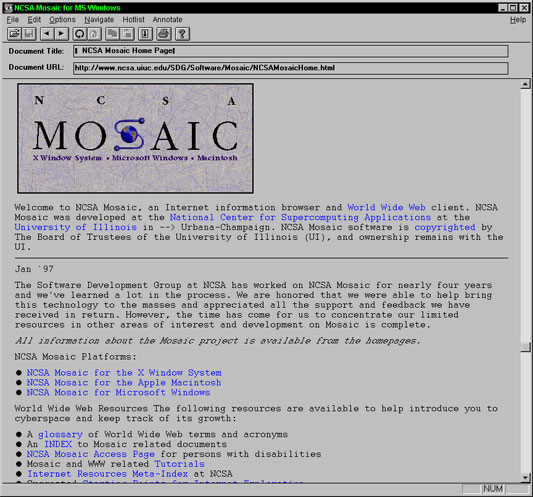
\includegraphics[scale=0.6]{imagens/mosaic_beta.jpg}
  \caption{NCSA Mosaic versão beta}
  \legend{Fonte: \cite{historyComputer}}
  \label{fig:historyComputer}
\end{figure}

O JavaScript foi introduzido em 1995 como uma forma de adicionar programas às 
páginas web do navegador Netscape. A linguagem, desde então, foi adotada por 
todos os outros grandes navegadores web que possuem interfaces gráficas. Ele 
tornou as aplicações modernas possíveis, fazendo com que você não tenha que 
recarregar a página inteira quando for necessário realizar interações diretas 
com a aplicação. Além disso, ele é usado em páginas web mais tradicionais, 
fornecendo diferentes maneiras de criar interatividade e inteligência \cite
{haverbeke2014eloquent}.

\section{ECMAScript ou JavaScript?}

Depois que o JavaScript foi adotado fora do Netscape, um documento padrão foi 
escrito para descrever a maneira na qual a linguagem deveria funcionar, 
garantindo que as diferentes partes dos softwares que afirmavam suportar 
JavaScript estavam, de fato, falando sobre a mesma linguagem. Esse documento é 
chamado de padrão ECMAScript, nomeado pela organização internacional Ecma, que 
foi responsável pela padronização. Na prática, os termos ECMAScript e 
JavaScript podem ser usados como sinônimos, pois são dois nomes para a mesma 
linguagem.

Na prática, existem diversos softwares que suportam JavaScript e possuem seu 
comportamente semelhante. Os navegadores, ou browsers, são exemplos destes 
tipos de software os quais implementam a linguagem por meio das especificações 
regidas pelo ECMAScript. Outro mais atual é o NodeJS ou simplesmente Node 
(https://nodejs.org/) que busca executar o JavaScript diretamente no servidor 
(Node será aprofundado em capítulos posteriores).

\section{Executando JavaScript}

Para constatar o fato citado na sessão anterior, vamos executar o seguinte código no console em diferentes navegadores. Para tanto, crie um arquivo \textbf{index.html} e um outro com o nome de \textbf{javascript.js}. No arquivo index.html adicione o seguinte código:

\begin{lstlisting}
  <!DOCTYPE HTML>
  <html lang="pt-br">
  <head>
      <meta charset="utf-8">
      <title>JS Exemplos</title>
  </head>
  <body>
    <script type="text/javascript" src="javascript.js"></script>
  </body>
  </html>
\end{lstlisting}

E no arquivo \textbf{javascript.js} adicione o seguinte:

\begin{lstlisting}
alert('Bem vindo(a) ao JavaScript')
\end{lstlisting}

O código acima possui o mesmo comportamento? Sim, o comportamento é o mesmo em todos os navegadores. Contudo, a forma gráfica com que é apresentado faz parte da implementação feita. Portanto, o desenvolvedor pode utilizar o JavaScript nos navegadores sem muito problema, pois eles seguem não ideias da equipe que o criou mas uma especificação que dita as regras de como determinadas funções devem se comportar.

\section{Versões do JavaScript ou edições ECMAScript}

Como foi visto, o ECMAScript é apenas a especificação. Contudo, ao estudar a 
linguagem é muito comum escutar a abreviação de ECMAScript, ou seja, ES. Assim, sempre que se ler ES seguido de um número, esse está fazendo referência a uma edição do ECMAScript. Atualmente, existem oito edições do ECMAScript publicadas, sendo que, a partir de 2015, as edições começaram a receber o ano e não mais o número da edição.

\begin{enumerate}
  \item ECMAScript 1 (1997)	
  \item ECMAScript 2 (1998)	
  \item ECMAScript 3 (1999)	
  \item ECMAScript 4	Nunca foi lançada.
  \item ECMAScript 5 (2009)
    \begin{enumerate}[label*=\arabic*.]
    \item ECMAScript 5.1 (2011)
    \end{enumerate}
  \item ECMAScript 2015
  \item ECMAScript 2016
  \item ECMAScript 2017
  \item ECMAScript 2018
\end{enumerate} 

\section{Conclusão}
Portanto, JavaScript se tornou a linguagem de programação mais popular no 
desenvolvimento Web sendo suportada por todos os navegadores e responsável por praticamente qualquer tipo de dinamismos em páginas web. Ao se usar todo o poder que ela tem para oferecer, pode-se chegar a resultados impressionantes. Alguns excelentes exemplos disso são aplicações Web complexas como Gmail, Google Maps e Google Docs. 
